By taking into consideration~\cite{lavalle2006planning}, we know we split the trajectory generation problem into 3 sub problems, path planning, trajectory optimization and velocity planning. During the first step we plan a path knowing only the geometrical configuration of the environment that goes from the initial to the desired configuration. This trajectory is then processed to be smoother and take into consideration the dynamics of the system, in the last sub problem we plan not only the velocity the agent should have during the trajectory, but also the reference actuation needed to follow the reference in an ideal situation. Using simple the first solution as the one used, where the dynamics are not considered is not acceptable as show in~\cite{bergman2021exploiting}, we can see a good example of this in figure \ref{eq: Proposed Approach: Space Cobot: Bad trajectory generation}, where the first path considered is not feasible due to the dynamics of the system.

\begin{figure}
    \centering
    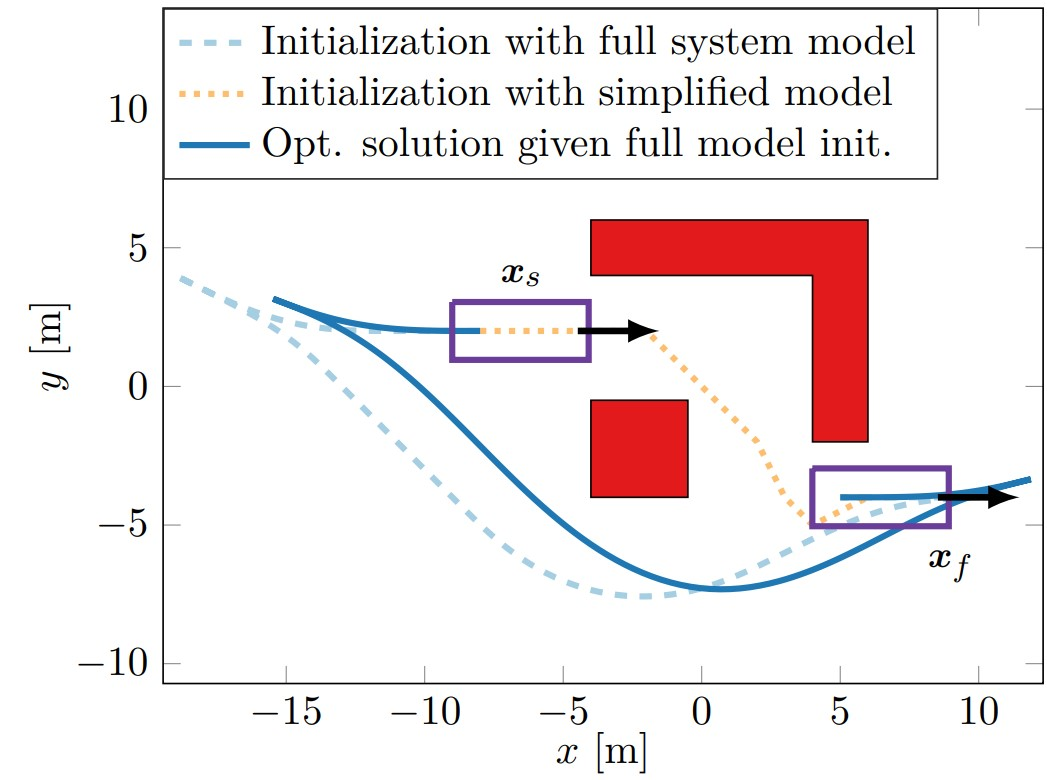
\includegraphics[width=0.7\textwidth]{Images/Propposed Aproach/bad_trajectory_generation.png}
    \caption{Example of a bad use of trajectory where the dynamics are not considered}
    \label{eq: Proposed Approach: Space Cobot: Bad trajectory generation}
\end{figure}

With this in mind, for the first step we will only plan the trajectory for the desired trajectory of the payload, since the payload is the objective, meaning we do not need to consider the other robots and their position. During the smoothing and dynamics consideration we can take into consideration the path that the robots will need to make sure the payload follows the desired trajectory. And lastly in the velocity planning we plan the velocity of the system, and the actuation each of the robots in the system will need to follow at each time step we can follow the trajectory plan in the last step. Due to the cooperative nature of the problem, there must be some consensus for the trajectory optimization step for all the robots, since neither can a single robot do all do work nor a robot not do work during the trajectory, this means during the optimization we need to optimize a single function, rather than have each robot optimizing its own trajectory. We can see the architecture for the trajectory generation of the system in figure \ref{fig:Proposed Approach: Trajectory Generation: Architecture}. The trajectory generated will then be used as the reference for the motion control algorithm used in the system.


\begin{figure}[H]
    \centering
    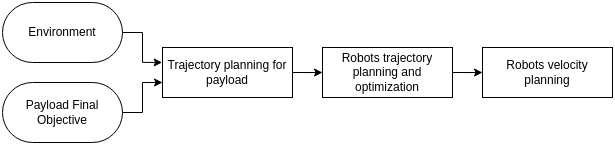
\includegraphics[width=0.7\textwidth]{Images/Propposed Aproach/System Motion planning.png}
    \caption{Trajectory Generation Architecture}
    \label{fig:Proposed Approach: Trajectory Generation: Architecture}
\end{figure}


